\section{Evaluation}

In all the experiments described in this section, we execute all drone flights at 2 meters per second, with a total travel budget of 960 meters (i.e., an 8 minute flight) unless otherwise noted.
All flights generate 1 image every 3.5 meters.
Each method has the same travel budget, and generates roughly 275 images.
Small variations in the number of generated images are possible, due to differences in how close each method gets to the travel budget.
We describe our drone hardware, data acquisition pipeline, and experimental methodology in more detail in Section \ref{sec:ch4:appendix}.

\begin{figure*}[t]
\begin{center}
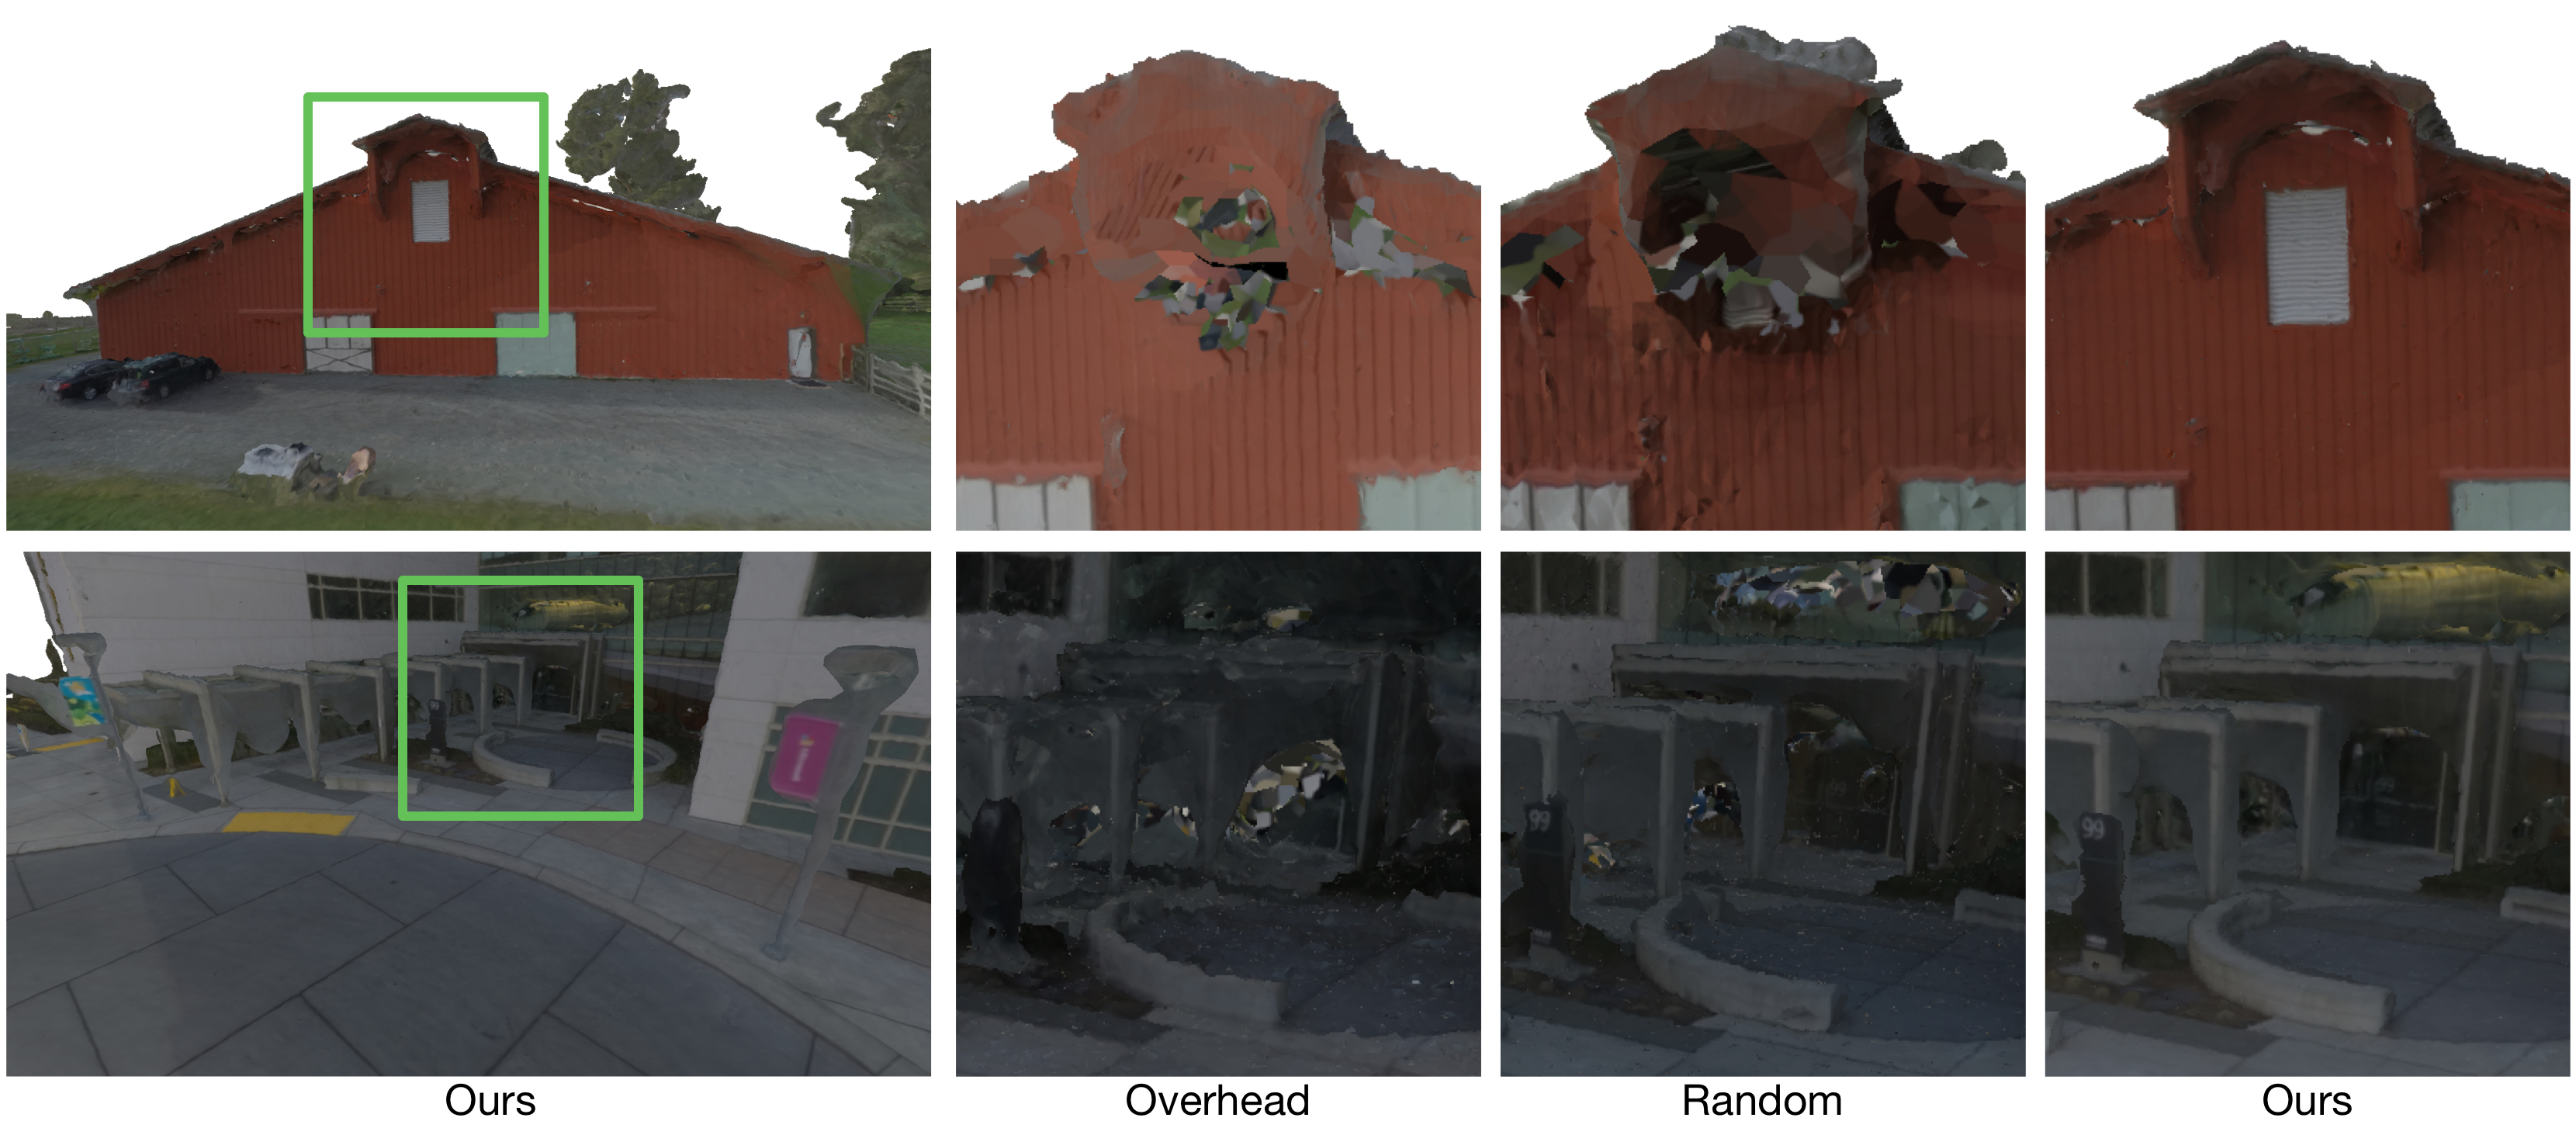
\includegraphics[width=6.0in]{images/2017_iccv/real_world_results.jpg}
\end{center}
\caption{
Qualitative comparison of the 3D reconstructions obtained from an overhead trajectory, a random trajectory, and our trajectory for two real-world scenes.
Our reconstructions contain noticeably fewer visual artifacts than the baseline reconstructions.
In all our experiments, we control for the flight time, battery consumption, number of images, and quality settings used in the 3D reconstruction.
}
\label{fig:ch4:results_side_by_side}
\end{figure*}

\paragraph{Real-World Reconstruction Performance}
We evaluated the real-world reconstruction performance of our algorithm by using it to scan three large outdoor scenes: a barn, an office building, and an industrial site.\footnote{We
conducted this experiment with an early implementation of our method that differs slightly from the implementation used in our other experiments.
In particular, the graph of camera positions used in this experiment included diagonal edges.
We subsequently excluded diagonal edges to enable our integer programming formulation to scale to larger problem instances. 
}
We show results from these experiments in Figures \ref{fig:ch1:teaser_ch4} and \ref{fig:ch4:results_side_by_side}, as well as in Section \ref{sec:ch4:eval_detail}.
We compared our reconstruction results to two baseline methods: \textsc{Overhead} and \textsc{Random}.

\textsc{Overhead}.
We designed \textsc{Overhead} to generate trajectories that are representative of those produced by existing commercial flight planning software \cite{3dr:2017a,pix4d:2017a}.
\textsc{Overhead} generates a single flight at at a safe height above the scene; consisting of an orbit path that always points the camera at the center of the scene; followed by a lawnmower path that always points the camera straight down.

\textsc{Random}.
We designed \textsc{Random} to have roughly the same level of scene understanding as our algorithm, except that \textsc{Random} does not optimize our coverage function.
We gave \textsc{Random} access to the graph of camera positions generated by our algorithm, which had been pruned according to the free space in the scene.
\textsc{Random} generates trajectories by randomly selecting graph nodes to visit and traveling to them via shortest paths, until no more nodes can be visited due to the travel budget.
\textsc{Random} always points the camera towards the center of the scene, which is a reasonable strategy for the scenes we consider in this chapter.

During our \emph{explore} phase, we generate an orbit trajectory exactly as we do for \textsc{Overhead}.
For the scenes we consider in this chapter, this initial orbit trajectory is always less than 250 meters.

When generating 3D\ reconstructions, our algorithm and \textsc{Random} have access to the images from our \emph{explore} phase, but \textsc{Overhead} does not.
The images in our \emph{explore} phase are nearly identical to the orbit images from \textsc{Overhead}, and would therefore provide \textsc{Overhead} with negligible additional information, so all three methods are directly comparable.
We generated 3D reconstructions using the commercially available Pix4Dmapper Pro software \cite{pix4d:2017b}, configured with maximum quality settings.

\begin{figure*}[t]
\begin{center}
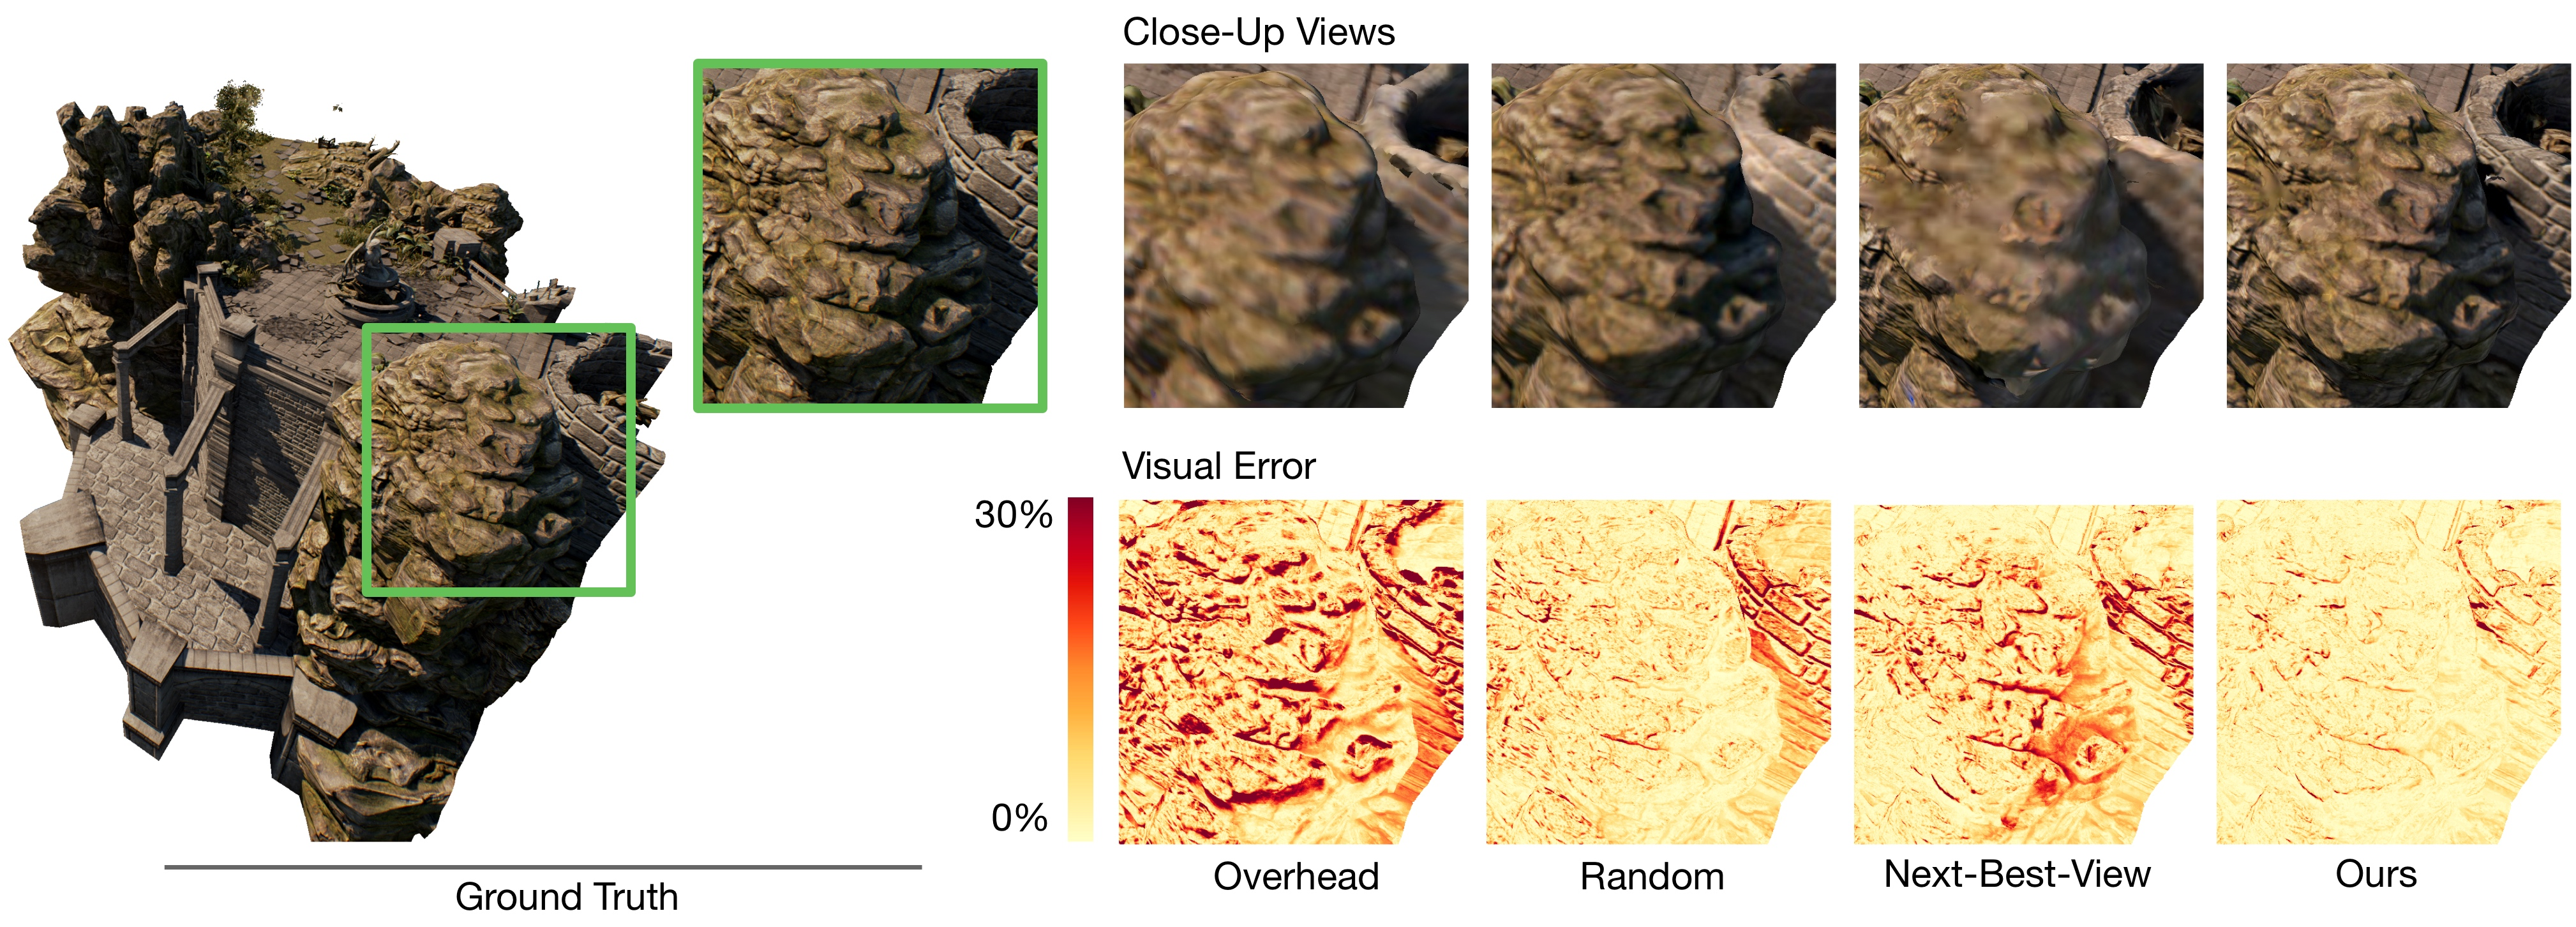
\includegraphics[width=6.0in]{images/2017_iccv/visual_error.jpg}
\end{center}
\caption{
Quantitative comparison of the 3D reconstructions obtained from an overhead trajectory, a random trajectory, a next-best-view trajectory, and our trajectory for our synthetic scene.
We show close-up renderings of each reconstruction, as well as per-pixel visual error, relative to a ground truth rendering of the scene.
Our method leads to quantitatively lower visual error than baseline methods.
}
\label{fig:ch4:results_quantitative}
\end{figure*}

\begin{table}[t]
\centering
\footnotesize
\begin{tabular}{@{}llll@{}}
\toprule
Method         & Accuracy       & Completeness   & Visual     \\
               & Error (mm)     & Error (mm)     & Error (\%) \\
\midrule
Overhead       & 170.2          & 583.8          & 7.1  \\
Random         & 126.5          & 557.2          & 4.4 \\
Next-Best-View & 122.8          & 330.7          & 3.6 \\
\textbf{Ours}  & \textbf{115.2} & \textbf{323.3} & \textbf{3.3} \\
\bottomrule
\end{tabular}
\normalsize
\caption{
Quantitative comparison of the 3D reconstructions obtained from an overhead trajectory, a random trajectory, a next-best-view trajectory, and our trajectory for our synthetic scene.
For all the columns in this table, lower is better.
We report the mean per-pixel visual error across all of our test views, where 100\% per-pixel error corresponds to the $l_2$ norm of the difference between black and white in RGB space.
Our method quantitatively outperforms baseline methods, both geometrically (i.e., in terms of accuracy and completeness) and visually.
}
\label{tbl:ch4:quantitative}
\end{table}

\paragraph{Reconstruction Performance on a Synthetic Scene}
We evaluated our algorithm using a photorealistic video game simulator, which
enabled us to measure reconstruction performance relative to known ground truth geometry and appearance.
We show results from this experiment in Figure \ref{fig:ch4:results_quantitative} and Table \ref{tbl:ch4:quantitative}.

Our experimental design here is exactly as described previously, except we acquired images by programmatically maneuvering a virtual camera in the Unreal Engine \cite{epic:2017a}, using the UnrealCV Python library \cite{qiu:2016}.
We also included an additional baseline method, \textsc{Next-Best-View}, that greedily selects nodes according to their marginal submodular reward, and finds an efficient path to connect them using the Approx-TSP algorithm \cite{cormen:2009} until no more nodes can be added due to the travel budget.
This method is intended to be representative of the \emph{next-best-view} planning strategies that occur frequently in the literature \cite{fan:2016,hollinger:2013,krainin:2011,wu:2014}, including those that have been applied to aerial 3D scanning \cite{dunn:2009a,hoppe:2012,mostegel:2016,schmid:2012}.

We chose the \textsc{Grass Lands} environment \cite{epic:2017b} as our synthetic test scene because it is freely available, has photorealistic lighting and very detailed geometry, and depicts a large outdoor scene that would be well-suited for 3D scanning with a drone.

We evaluated geometric reconstruction quality by measuring \emph{accuracy} and \emph{completeness} relative to a ground truth point cloud \cite{aanaes:2016,knapitsch:2017}.
We obtained our ground truth point cloud by rendering reference depth images arranged on an inward-looking sphere around the scene, taking care to manually remove any depth images that were inside objects.
We also evaluated visual reconstruction quality by measuring \emph{per-pixel visual error}, relative to ground truth RGB images rendered from the same inward-looking sphere around the scene \cite{waechter:2017}.
When evaluating per-pixel visual error, we took care to only compare pixels that contain geometry from inside the scanning region-of-interest for our scene.

When evaluating geometric quality, we obtained point clouds for each method by running VisualSFM \cite{wu:2013,wu:2007,wu:2011b,wu:2011a}, followed by the Multi-View Environment \cite{fuhrmann:2015}, followed by Screened Poisson Surface Reconstruction \cite{kazhdan:2013}, and finally by uniformly sampling points on the reconstructed triangle mesh surface.
When evaluating visual quality, we obtained textured 3D models for each method using the surface texturing algorithm of Waechter et al.~\cite{waechter:2014}.


\begin{figure}[t]
\begin{center}
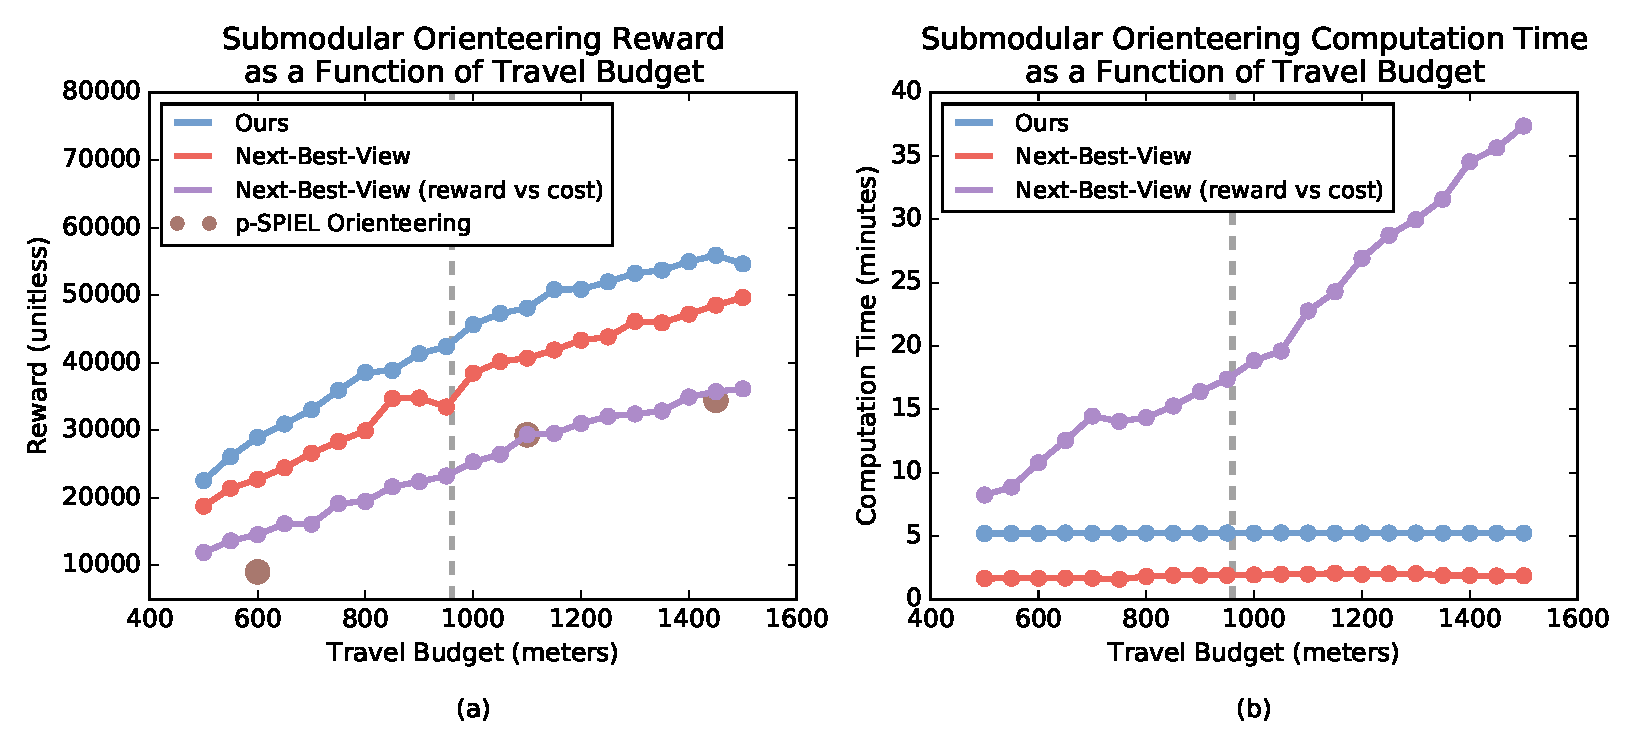
\includegraphics[width=4.0in]{images/2017_iccv/00_quantitative.pdf}
\end{center}
\caption{
Quantitative comparison of submodular orienteering algorithms on our synthetic scene.
(a) Submodular reward as a function of travel budget.
Our algorithm consistently obtains more reward than other algorithms.
%, across a range of different travel budgets.
All reconstruction results in this chapter were produced with a budget of 960 meters (i.e., 8 minutes at 2 meters per second), shown with a grey dotted line.
For this budget, we obtain 20\% more reward than next-best-view planning. The p-SPIEL Orienteering algorithm \cite{singh:2009b} failed to consistently find a solution.
(b) Computation time as a function of travel budget.
On this plot, lower is better.
In terms of computation time, our algorithm is competitive with, but more expensive than, next-best-view planning.
We do not show computation times for the p-SPIEL Orienteering algorithm, because it took over 4 hours in all cases where it found a solution.
}
\label{fig:ch4:results_orienteering}
\end{figure}

\paragraph{Submodular Orienteering Performance}
We evaluated the submodular orienteering performance of our algorithm on our synthetic scene.
We performed this experiment after we have solved for the optimal camera orientation at every node in our graph, to facilitate the comparison of our algorithm to other submodular orienteering algorithms \cite{singh:2009b,zhang:2016}.
We show results from this experiment in Figure \ref{fig:ch4:results_orienteering}.

In this experiment, we included a baseline method that behaves identically to \textsc{Next-Best-View}, except it greedily selects nodes according to the ratio of marginal reward to marginal cost \cite{zhang:2016}.
We implemented all algorithms in Python, except for the p-SPIEL Orienteering algorithm \cite{singh:2009b}, where we used the MATLAB implementation provided by the authors.
We performed this experiment on a Mid 2015 Macbook Pro with a 2.8 GHz Intel Core i7 processor and 16GB of RAM.

%\begin{figure}[t]
%\begin{center}
%\includegraphics[width=0.47\textwidth]{figures/01_quantitative.pdf}
%\end{center}
%\caption{
%Comparing computation times of the Greedy and Lazy Greedy algorithms for submodular subset selection, for our real-world scenes.
%Smaller bars are better.
%For all our scenes, the Lazy Greedy algorithm is more than 450$\times$ faster than the Greedy algorithm, and achieves the same amount of submodular reward.
%}
%\label{fig:results_side_by_side}
%\end{figure}


